\newpage
\section{Background}\label{background}
\subsection{Principles of Cellular Automata}\label{CA_Principles}

A cellular automaton (CA) is a discrete model of cells arranged in a grid that possesses a set of given states. The state of each cell evolves over a series of time steps according to a set of rules that depend on the states of neighbouring cells. These rules can be applied as many times as required, simulating the evolution of a system over time. \newline \indent In the 1980s, Stephen Wolfram conducted comprehensive studies into elementary cellular automata. An elementary CA works based on two possible states, represented by either a 0 or a 1. Wolfram found that there are 256 different possible rules for elementary CA, each of which is indexed by a unique binary number \cite{wolfram1986theory}. Despite the simplicity of the model, rule number 30 exhibits chaotic behaviour, and can be used as a random number generator \cite{Wolfram_2002}. In Figure \ref{rule190} we observe the elementary cellular automaton for Wolfram's rule 190.

\begin{figure}[h!]
\centering
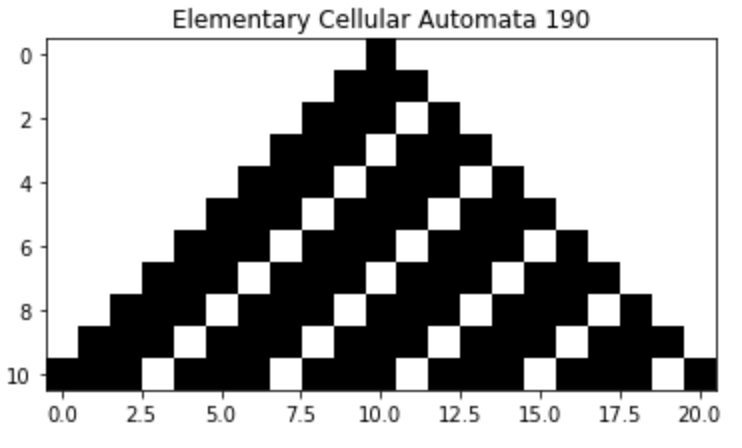
\includegraphics[width=0.5\textwidth]{Figures/cell.png}\caption{An example of an elementary CA using Wolfram's rule 190 for 10 time steps \cite{wolfram1986theory}. White squares represent 0 and black squares represent 1. Each horizontal line represents a different time step, with the initial time step having a '1' binary state at position 10.0 on the x-axis.}\label{rule190}
\end{figure} 

\noindent Cellular automata can be defined in arbitrarily many dimensions. A two-dimensional CA is composed of a rectangular grid of cells; the state of each cell is updated in discrete time steps depending on a particular rule set. The collection of cells surrounding any particular cell is known as the neighbourhood, and the values of the neighbourhood determine the future state of a cell. Two commonly used  neighbourhoods in 2D cellular automata are the \textit{von Neumann neighbourhood} \cite{wolfram1986theory} and the \textit{Moore neighbourhood} \cite{101917}, illustrated in Figure \ref{hoods}. The former is composed of a central cell and the 4 cells adjacent to it, while the latter is composed of a central cell and the 8 cells surrounding it.\newline \indent The advantage of a small neighbourhood is computation speed: there are $50\%$ fewer values required to look up in the von Neumann neighbourhood compared to the Moore neighbourhood. Alternatively, the benefit of a larger neighbourhood is a greater number of possible combinations of cell values. The Moore neighbourhood includes the whole surroundings of a cell, and thus it can model movement in all directions \cite{Quartieri_2010}.

\begin{figure}[h!]
\begin{center}
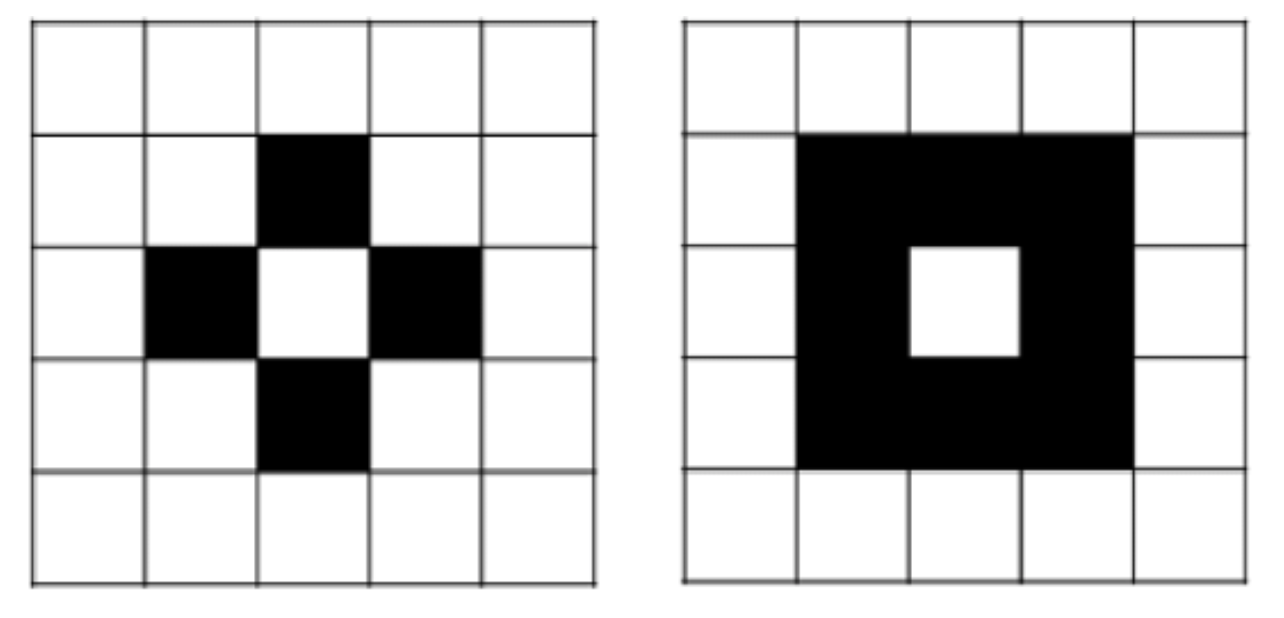
\includegraphics[width=0.5\textwidth]{Figures/von.png}\caption{Cell neighbourhoods visualised in a 2D array, neighbour cells highlighted in black. Left: the von Neumann neighbourhood. Right: the Moore neighbourhood.}\label{hoods}
\end{center}
\end{figure} 

\subsection{Modelling Wildfire}\label{Modelling_Wildfire}

A wildfire is defined as an uncontrolled fire in a rural area with combustible vegetation \cite{press2008cambridge}. Our primary objective is to recreate behaviour exhibited by wildfires for a given environment, thus describing the evolution of the fires and making accurate predictions of their future state. \newline \indent Classical methods of mathematical wildfire models include empirical and physically-based models. Empirical fire models are based on experience and intuition from past fires, while physically-based models are formulated around a fundamental conservation law of physics. For example, certain wildfire models can reproduce the relationship between the rate of fire spread and the amount of heat generated by the fires \cite{nobel_1980}, using the thermodynamic process of burning to describe the physical system of an evolving wildfire. Such classical models are often based on computationally intensive mathematics, such as hyperbolic diffusion-reaction equations \cite{1997PhRvE..56.6557M} or stochastic differential equations \cite{rothermel1972mathematical}. \newline \indent
An alternative approach to fire modelling uses a rule-based CA model with probabilistic effects. CA models are good candidates for modelling dynamical systems whose evolution depends on microscopic interactions of their constituent parts, because the interactions can be directly programmed into the rules of evolution of the cell array. The properties of CA systems are a possible representation of a wildfire system, where the fire propagation rate, fire spreading direction and the fire duration are mainly dependent on local characteristics such as vegetation, gradient and relative humidity. Cellular automaton models can incorporate these local characteristics within a theoretical fire spread mechanism, and past CA models have yielded positive results in replicating real wildfires \cite{inproceedings}.\newline \indent
Our objective is to model the 2009 Australian bushfires in the Shire of Murrindindi using cellular automata. A cell-based model is more appropriate for a simulation of this size, as finding solutions to physically-based models at the scale of $150 \times 100$ km is computationally unfeasible. The rules incorporated into our model are an adaptation of those developed by A. Aleksandridis \textit{et al.} in 2008 \cite{Aleksandridis_2008} as well as A. Quartieri \textit{et al.} in 2010 \cite{Quartieri_2010}. We incorporate the environmental factors of wind, elevation and embers into the model, and use real geographical data from the region to simulate the conditions of fire at the time of the events.